\chapter{Methodology Results and Discussion}

Materials and Methods is the chronological listing of steps and procedure/s used by the proponent/s.
Methods used for gathering of data, laboratory and field experiment, theoretical and/or conceptual frameworks, as well as techniques employed in the analyses of data must be specifically listed.

\section{Software Design}

The software design of Proctor Vue is represented by the following Hierarchical Input-Process-Output (HIPO) diagrams.

\vspace{1cm}

\begin{figure}[h!]
    \begin{center}
        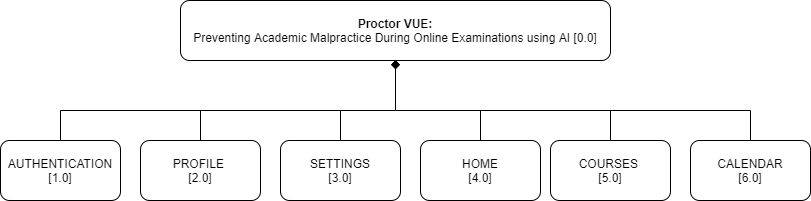
\includegraphics[scale=0.5]{main-hipo}
        \caption{Sample of HIPO}
    \end{center}
\end{figure}

\begin{figure}[h!]
    \begin{center}
        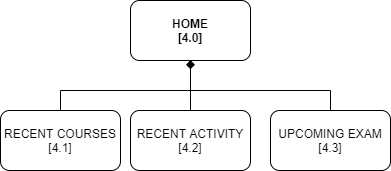
\includegraphics[scale=0.7]{home-hipo.png}
        \caption{Home Page}
    \end{center}
\end{figure}

\vspace{1cm}

\begin{figure}[h!]
    \begin{center}
        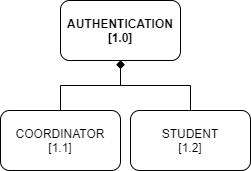
\includegraphics[scale=0.7]{auth-hipo.png}
        \caption{Authentication}
    \end{center}
\end{figure}

\begin{figure}[h!]
    \begin{center}
        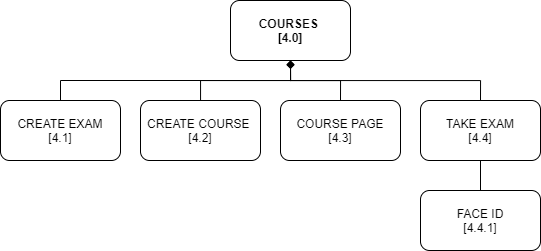
\includegraphics[scale=0.7]{courses-hipo.png}
        \caption{Courses}
    \end{center}
\end{figure}

\section{System Architecture}

\section{Conceptual Design}

\section{Cost Benefit Analysis}

\section{Requirement Analysis}

\section{Block Diagrams}

\section{Development and Testing}

\section{Input and Output Reports and Analysis}

\section{Description of the Prototype}

\section{Implementation Plan}

\section{Algorithm Use}

Proctor Vue utilizes an open source high-level face detection library, \lstinline{face-api.js}.
Under the hood, the library implements facial detection and recognition, as well as other useful functions such as age and gender recognition which are unused in Proctor Vue, using different machine learning algorithms to cater to different use cases.
The researchers wanted to have the most seamless and optimized experience during the exams so they opted to use the pre-trained tiny face detector model for the app's purposes.

The Tiny Face Detector model, unlike other well-known face detection models, is faster and more optimized, especially for detecting smaller faces out of a large image.
It makes intuitive use of different factors such as scale, resolution, and context for object detection.
In a research made by the original developers of the model, they found that the model can detect approximately 80\% of 1000 faces in a large image \cite{Hu_2017_CVPR}.

The facial recognition model, under the hood, is implemented using a residual network.
In practice, it will compute a descriptor for a person's face, describing their face's unique characteristics.
The model has an accuracy of 99.38\% in a facial recognition benchmark test.
